\section{Introduction}

\paragraph{Premise: error compounds along the horizon, and chunk length is how
a policy trades against it.}
Imitation-learned manipulation policies increasingly predict chunks of actions
rather than single steps \citep{zhao2023act,chi2023diffusion}. A chunked
executor plays $k$ actions open-loop and then replans. The reason to make $k$
large is that replanning at every step is expensive, adds dithering, and is
often unnecessary. The reason to keep $k$ small is the classical one: a policy
that acts without observing accumulates error, and in imitation learning that
error compounds along the horizon rather than staying bounded
\citep{ross2010efficient,ross2011dagger}. Chunk length is therefore a direct
control on how much compounding the executor allows between observations.

How fast error actually compounds is a property of the dynamics at the current
state, and it has a standard measurement. If a small perturbation is injected
and the system is run forward, the exponential rate at which the perturbed and
unperturbed trajectories separate over a finite window is a finite-time
maximal Lyapunov exponent \citep{haller2015lcs}, a tool already used to
diagnose the sensitivity of model predictive control and reinforcement
learning policies \citep{krishna2023ftle}. We write this rate $\lambda$ and use
it as the definition of open-loop stability for a chunk. A segment with
$\lambda$ below a task-specific floor is open-loop stable, meaning a
perturbation dies out while the chunk plays; a segment above it is open-loop
unstable, meaning every additional blind step makes the error larger.

Existing methods that vary the execution horizon do not measure this quantity.
They trigger on model confidence, on attention weights, on entropy, on the
consistency of successive chunk samples, or on the kinematics of the predicted
path \citep{zhao2026dehp,wang2026autohorizon,nie2026pace,zhang2026hipolicy,feng2026dvac,so2025sgac}.
Those are proxies for how sure the policy is, not for how fast the plant
amplifies an error. This paper studies the quantity itself.

\paragraph{The three parts of this paper.}
The paper makes three claims and reports the evidence for each separately,
including where that evidence is still incomplete.
Figure~\ref{fig:framework} states all three in one picture.

% Framework figure: the three claims of the paper in one picture.
%
% Panel (a) is real data, not a schematic:
%   /mnt/scratch/lh/labels/final3_env_rc_PickPlaceCounterToCabinet.npz, demo 20.
%   lambda_task at stride 2, delta = .0649 (the automatic per-task threshold).
%   The adaptive ribbon is the (16,1) rule of Sec. 3 run on that trace.
% Panel (c) uses the measured median lambda of that same task,
%   .0798 on unstable stamps and .0030 on stable ones; the implied 24-step
%   growth exp(24 lambda) = 6.8x and 1.07x matches the measured median
%   d_last/d_first of 6.57x and 1.14x.

\definecolor{cstable}{RGB}{46,110,175}
\definecolor{cunstable}{RGB}{198,55,45}
\definecolor{cband}{RGB}{250,224,219}
\definecolor{cbox}{RGB}{241,243,246}
\definecolor{cline}{RGB}{88,94,104}
\definecolor{coracle}{RGB}{116,102,178}

\begin{figure}[t]
\centering

%% ---------------------------------------------------------------- panel (a)
\begin{tikzpicture}[font=\footnotesize]
\begin{axis}[
  name=lam, scale only axis, width=11.9cm, height=2.5cm,
  xmin=0, xmax=170, ymin=-0.115, ymax=0.155,
  xticklabels={}, xtick={0,20,40,60,80,100,120,140,160},
  ytick={-0.1,0,0.1}, yticklabel style={font=\scriptsize},
  ylabel={$\lambda$}, ylabel style={font=\footnotesize, yshift=-6pt},
  axis line style={cline}, tick style={cline},
  every axis plot/.append style={line width=0.9pt},
  clip mode=individual,
]
  % unstable bands (lambda > delta), widened by one stride for visibility
  \fill[cband] (axis cs:47,-0.115) rectangle (axis cs:49,0.155);
  \fill[cband] (axis cs:51,-0.115) rectangle (axis cs:53,0.155);
  \fill[cband] (axis cs:61,-0.115) rectangle (axis cs:69,0.155);
  \fill[cband] (axis cs:151,-0.115) rectangle (axis cs:155,0.155);
  % automatic threshold
  \draw[cunstable, dashed, line width=0.7pt]
    (axis cs:0,0.0649) -- (axis cs:170,0.0649);
  \node[cunstable, font=\scriptsize, anchor=west]
    at (axis cs:171,0.0649) {$\delta$};
  \addplot[cstable, smooth] coordinates {
    (0,-0.0663) (2,0.0194) (4,0.0266) (6,0.0180) (8,0.0101) (10,0.0058) (12,-0.0011) (14,-0.0083)
    (16,-0.0038) (18,-0.0060) (20,-0.0129) (22,-0.0151) (24,-0.0437) (26,-0.0264) (28,-0.0087) (30,-0.0071)
    (32,-0.0040) (34,-0.0114) (36,-0.0097) (38,-0.0075) (40,-0.0297) (42,-0.0599) (44,-0.0670) (46,0.0110)
    (48,0.1208) (50,0.0410) (52,0.0660) (54,0.0410) (56,0.0533) (58,0.0518) (60,0.0518) (62,0.0775)
    (64,0.1000) (66,0.0670) (68,0.0706) (70,0.0249) (72,0.0117) (74,0.0116) (76,0.0073) (78,0.0051)
    (80,0.0005) (82,-0.0039) (84,-0.0163) (86,-0.0170) (88,-0.0204) (90,-0.0386) (92,-0.0390) (94,-0.0731)
    (96,-0.0499) (98,-0.0295) (100,-0.0152) (102,-0.0075) (104,0.0075) (106,0.0123) (108,0.0146) (110,0.0165)
    (112,0.0369) (114,0.0415) (116,0.0236) (118,0.0129) (120,0.0040) (122,0.0088) (124,0.0091) (126,-0.0028)
    (128,-0.0157) (130,-0.0415) (132,-0.0560) (134,-0.0947) (136,-0.0782) (138,-0.0659) (140,-0.0332) (142,-0.0153)
    (144,0.0183) (146,0.0271) (148,0.0554) (150,0.0532) (152,0.0670) (154,0.0805) (156,0.0336) (158,0.0413)
    (160,0.0265) (162,0.0142) (164,0.0213) (166,0.0230) (168,0.0072) (170,0.0027)
  };
  \node[anchor=north west, font=\scriptsize, cline, align=left]
    at (axis cs:2,0.152) {open-loop stable};
  \node[anchor=north, font=\scriptsize, cunstable, align=center]
    at (axis cs:65,0.152) {unstable};
\end{axis}

%% chunk-length ribbons, sharing the x axis of the plot above
\begin{axis}[
  at={(lam.below south west)}, anchor=north west, yshift=-2pt,
  scale only axis, width=11.9cm, height=1.35cm,
  xmin=0, xmax=170, ymin=-0.55, ymax=2,
  xtick={0,20,40,60,80,100,120,140,160},
  xlabel={control step $t$ within one episode},
  xlabel style={font=\footnotesize, yshift=2pt},
  ticklabel style={font=\scriptsize},
  ytick={0.5,1.5}, yticklabels={adaptive $k$, fixed $k{=}16$},
  y tick label style={font=\scriptsize, align=right},
  axis line style={cline}, tick style={cline}, ytick style={draw=none},
  tick align=outside, clip mode=individual,
]
  \fill[cband] (axis cs:47,-0.55) rectangle (axis cs:49,2);
  \fill[cband] (axis cs:51,-0.55) rectangle (axis cs:53,2);
  \fill[cband] (axis cs:61,-0.55) rectangle (axis cs:69,2);
  \fill[cband] (axis cs:151,-0.55) rectangle (axis cs:155,2);

  % fixed k=16: every chunk is the same length, four of them run blind
  % straight through an unstable band
  \draw[fill=cstable!22, draw=cstable, line width=0.5pt] (axis cs:0,1.18) rectangle (axis cs:16,1.82);
  \draw[fill=cstable!22, draw=cstable, line width=0.5pt] (axis cs:16,1.18) rectangle (axis cs:32,1.82);
  \draw[fill=cstable!22, draw=cstable, line width=0.5pt] (axis cs:32,1.18) rectangle (axis cs:48,1.82);
  \draw[fill=cstable!22, draw=cstable, line width=0.5pt] (axis cs:48,1.18) rectangle (axis cs:64,1.82);
  \draw[fill=cstable!22, draw=cstable, line width=0.5pt] (axis cs:64,1.18) rectangle (axis cs:80,1.82);
  \draw[fill=cstable!22, draw=cstable, line width=0.5pt] (axis cs:80,1.18) rectangle (axis cs:96,1.82);
  \draw[fill=cstable!22, draw=cstable, line width=0.5pt] (axis cs:96,1.18) rectangle (axis cs:112,1.82);
  \draw[fill=cstable!22, draw=cstable, line width=0.5pt] (axis cs:112,1.18) rectangle (axis cs:128,1.82);
  \draw[fill=cstable!22, draw=cstable, line width=0.5pt] (axis cs:128,1.18) rectangle (axis cs:144,1.82);
  \draw[fill=cstable!22, draw=cstable, line width=0.5pt] (axis cs:144,1.18) rectangle (axis cs:160,1.82);
  \draw[fill=cstable!22, draw=cstable, line width=0.5pt] (axis cs:160,1.18) rectangle (axis cs:170,1.82);
  \draw[draw=cunstable, line width=0.9pt] (axis cs:32,1.18) rectangle (axis cs:48,1.82);
  \draw[draw=cunstable, line width=0.9pt] (axis cs:48,1.18) rectangle (axis cs:64,1.82);
  \draw[draw=cunstable, line width=0.9pt] (axis cs:64,1.18) rectangle (axis cs:80,1.82);
  \draw[draw=cunstable, line width=0.9pt] (axis cs:144,1.18) rectangle (axis cs:160,1.82);

  % adaptive: the (16,1) rule executed on this trace
  \draw[fill=cstable!22, draw=cstable, line width=0.5pt] (axis cs:0,0.18) rectangle (axis cs:16,0.82);
  \draw[fill=cstable!22, draw=cstable, line width=0.5pt] (axis cs:16,0.18) rectangle (axis cs:32,0.82);
  \draw[fill=cstable!22, draw=cstable, line width=0.5pt] (axis cs:32,0.18) rectangle (axis cs:48,0.82);
  \draw[fill=cstable!22, draw=cstable, line width=0.5pt] (axis cs:50,0.18) rectangle (axis cs:66,0.82);
  \draw[fill=cstable!22, draw=cstable, line width=0.5pt] (axis cs:70,0.18) rectangle (axis cs:86,0.82);
  \draw[fill=cstable!22, draw=cstable, line width=0.5pt] (axis cs:86,0.18) rectangle (axis cs:102,0.82);
  \draw[fill=cstable!22, draw=cstable, line width=0.5pt] (axis cs:102,0.18) rectangle (axis cs:118,0.82);
  \draw[fill=cstable!22, draw=cstable, line width=0.5pt] (axis cs:118,0.18) rectangle (axis cs:134,0.82);
  \draw[fill=cstable!22, draw=cstable, line width=0.5pt] (axis cs:134,0.18) rectangle (axis cs:150,0.82);
  \draw[fill=cstable!22, draw=cstable, line width=0.5pt] (axis cs:150,0.18) rectangle (axis cs:166,0.82);
  \draw[fill=cstable!22, draw=cstable, line width=0.5pt] (axis cs:166,0.18) rectangle (axis cs:170,0.82);
  \draw[fill=cunstable, draw=cunstable, line width=0.4pt] (axis cs:48,0.18) rectangle (axis cs:49,0.82);
  \draw[fill=cunstable, draw=cunstable, line width=0.4pt] (axis cs:49,0.18) rectangle (axis cs:50,0.82);
  \draw[fill=cunstable, draw=cunstable, line width=0.4pt] (axis cs:66,0.18) rectangle (axis cs:67,0.82);
  \draw[fill=cunstable, draw=cunstable, line width=0.4pt] (axis cs:67,0.18) rectangle (axis cs:68,0.82);
  \draw[fill=cunstable, draw=cunstable, line width=0.4pt] (axis cs:68,0.18) rectangle (axis cs:69,0.82);
  \draw[fill=cunstable, draw=cunstable, line width=0.4pt] (axis cs:69,0.18) rectangle (axis cs:70,0.82);
  \node[anchor=north, font=\scriptsize, cunstable] at (axis cs:100,0.10)
    {$k{=}1$ at the six steps judged unstable};
\end{axis}
\node[anchor=north west, font=\footnotesize\bfseries]
  at ($(lam.north west)+(-0.85cm,0.30cm)$) {(a)};
\end{tikzpicture}

\vspace{4pt}

%% ---------------------------------------------------------------- panel (b)
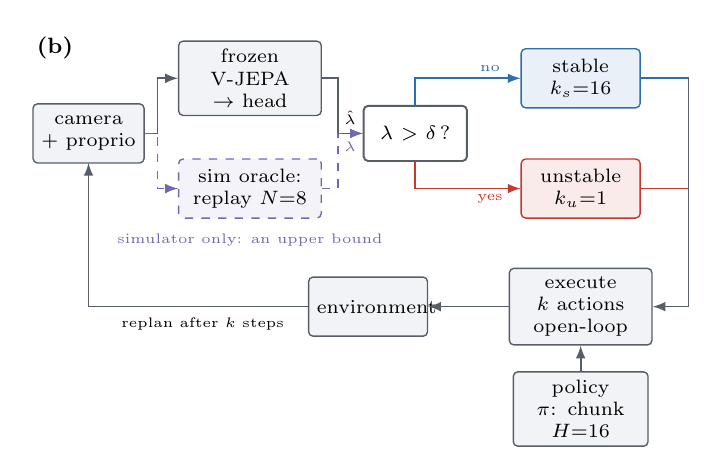
\begin{tikzpicture}[font=\scriptsize,
  box/.style={draw=cline, fill=cbox, rounded corners=1.6pt, align=center,
              inner sep=3pt, minimum height=7.5mm, line width=0.5pt},
  dec/.style={draw=cline, fill=white, rounded corners=1.6pt, align=center,
              inner sep=3pt, minimum height=7mm, line width=0.7pt},
  ar/.style={-latex, cline, line width=0.6pt},
]
% --- score the current state ------------------------------------------
\node[box, text width=12mm] (obs) at (0,1.05) {camera\\+ proprio};
\node[box, text width=16mm] (enc) at (2.05,1.75)
  {frozen V-JEPA $\rightarrow$ head};
\node[box, text width=16mm, draw=coracle, fill=coracle!8, dashed]
  (orc) at (2.05,0.35) {sim oracle: replay $N{=}8$};
\node[dec, text width=11mm] (cmp) at (4.15,1.05) {$\lambda > \delta$\,?};
% --- pick the chunk length --------------------------------------------
\node[box, text width=13mm, draw=cstable, fill=cstable!10]
  (ks) at (6.25,1.75) {stable\\ $k_s{=}16$};
\node[box, text width=13mm, draw=cunstable, fill=cunstable!10]
  (ku) at (6.25,0.35) {unstable\\ $k_u{=}1$};
% --- execute (row runs right to left, so the loop closes at the camera) -
\node[box, text width=16mm] (exe) at (6.25,-1.15)
  {execute $k$ actions open-loop};
\node[box, text width=13mm] (env) at (3.55,-1.15) {environment};
\node[box, text width=15mm] (pol) at (6.25,-2.45)
  {policy $\pi$: chunk $H{=}16$};

\draw[ar] (obs.east) -- ++(0.16,0) |- (enc.west);
\draw[ar, coracle, dashed] (obs.east) -- ++(0.16,0) |- (orc.west);
\draw[ar] (enc.east) -- ++(0.20,0) |- (cmp.west);
\draw[ar, coracle, dashed] (orc.east) -- ++(0.20,0) |- (cmp.west);
\node[anchor=south east, inner sep=1pt, font=\tiny] at (3.44,1.12)
  {$\hat\lambda$};
\node[anchor=north east, inner sep=1pt, font=\tiny, coracle] at (3.44,0.98)
  {$\lambda$};

\draw[ar, cstable] (cmp.north) |- (ks.west);
\draw[ar, cunstable] (cmp.south) |- (ku.west);
\node[anchor=south, inner sep=1pt, font=\tiny, cstable] at (5.10,1.79) {no};
\node[anchor=north, inner sep=1pt, font=\tiny, cunstable] at (5.10,0.31)
  {yes};
% both branches leave to the right of the boxes, then drop to the exec row
\draw[cstable, line width=0.6pt] (ks.east) -- (7.62,1.75);
\draw[cunstable, line width=0.6pt] (ku.east) -- (7.62,0.35);
\draw[ar] (7.62,1.75) -- (7.62,-1.15) -- (exe.east);
\draw[ar] (pol.north) -- (exe.south);
\draw[ar] (exe.west) -- (env.east);
\draw[ar] (env.west) -| (0,0.675);
\node[anchor=north, font=\tiny, inner sep=2pt] at (1.45,-1.22)
  {replan after $k$ steps};

\node[anchor=north west, font=\footnotesize\bfseries] at (-0.78,2.40) {(b)};
\node[anchor=north, font=\tiny, coracle] at (2.05,-0.10)
  {simulator only: an upper bound};
\end{tikzpicture}
\hfill
%% ---------------------------------------------------------------- panel (c)
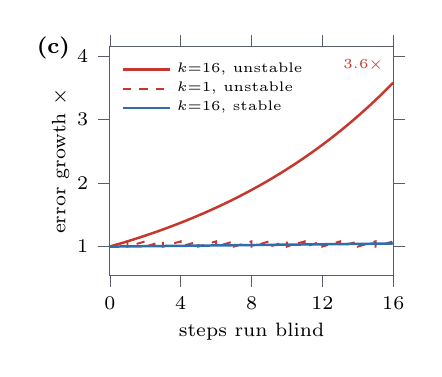
\begin{tikzpicture}[font=\footnotesize]
\begin{axis}[
  scale only axis, width=3.6cm, height=2.9cm,
  xmin=0, xmax=16, ymin=0.55, ymax=4.15,
  xtick={0,4,8,12,16}, ytick={1,2,3,4},
  ticklabel style={font=\scriptsize},
  xlabel={steps run blind}, ylabel={error growth $\times$},
  xlabel style={font=\scriptsize, yshift=2pt},
  ylabel style={font=\scriptsize, yshift=-4pt},
  axis line style={cline}, tick style={cline}, tick align=outside,
  every axis plot/.append style={line width=0.9pt},
  legend style={at={(0.03,0.97)}, anchor=north west, font=\tiny,
                draw=none, fill=none, cells={anchor=west}, row sep=-2pt,
                inner sep=1pt},
  legend cell align=left, clip mode=individual,
]
  \addplot[cunstable, domain=0:16, samples=60] {exp(0.0798*x)};
  \addlegendentry{$k{=}16$, unstable}
  \node[anchor=south east, font=\tiny, cunstable] at (axis cs:16,3.62)
    {$3.6\times$};
  \addplot[cunstable, dashed, line width=0.7pt] coordinates {
    (0,1) (1,1.083) (1,1) (2,1.083) (2,1) (3,1.083) (3,1) (4,1.083) (4,1)
    (5,1.083) (5,1) (6,1.083) (6,1) (7,1.083) (7,1) (8,1.083) (8,1)
    (9,1.083) (9,1) (10,1.083) (10,1) (11,1.083) (11,1) (12,1.083) (12,1)
    (13,1.083) (13,1) (14,1.083) (14,1) (15,1.083) (15,1) (16,1.083)
  };
  \addlegendentry{$k{=}1$, unstable}
  \addplot[cstable, domain=0:16, samples=2] {exp(0.0030*x)};
  \addlegendentry{$k{=}16$, stable}
\end{axis}
\node[anchor=north west, font=\footnotesize\bfseries] at (-1.05,3.15) {(c)};
\end{tikzpicture}

\caption{\textbf{The framework and the three claims.}
\textbf{(a)} Open-loop divergence rate $\lambda$ along one real
PickPlaceCounterToCabinet episode, with the automatic threshold $\delta$ and
the unstable segments shaded. Both regimes occur inside this single episode,
which contains four separate unstable segments; that is the ordinary case, as
78 to 96 percent of RoboCasa episodes contain both. The ribbons below show what
a chunk length can do about it. A fixed $k{=}16$ schedule is blind to the regime, and
four of its eleven chunks (red outline) run straight through an unstable
segment. The adaptive schedule is the $(16,1)$ rule of Section~\ref{sec:method}
executed on this trace: it keeps the long chunk in stable stretches, where a
long chunk costs nothing, and drops to $k{=}1$ only at the six steps it judges
unstable.
\textbf{(b)} The controller. At each replan a stability score is obtained
either from a learned head reading camera frames and proprioception, which is
what a real robot can do, or from a simulator oracle that measures $\lambda$ by
saving the state, replaying the proposed chunk once unperturbed and $N{=}8$
times perturbed, and rewinding. The score is compared to $\delta$ and selects
the chunk length; everything else in the loop is unchanged.
\textbf{(c)} Why the regime has to be known. Growth of the perturbation over a
chunk at the measured median rates for this task, $\lambda{=}.080$ on unstable
stamps and $.003$ on stable ones. Running blind through an unstable segment
compounds error by $3.6\times$ over 16 steps, while the same 16 blind steps in a
stable segment cost $1.05\times$; replanning every step holds the unstable case
at $1.08\times$. Over the full $K{=}24$ label window the measured divergence
ratio is $6.6\times$ to $14\times$ on unstable stamps against $0.97\times$ to
$1.4\times$ on stable ones across the four tasks. A single chunk length must
pay the first cost everywhere or give up the second everywhere.}
\label{fig:framework}
\end{figure}


\textbf{Claim 1: a single task contains both regimes, so a single chunk length
per task is the wrong unit.} Error does not compound at a uniform rate along
an episode. We measure $\lambda$ at every timestep of more than twenty datasets
on three platforms, and find that between 78 and 100 percent of individual
episodes contain both open-loop stable and open-loop unstable segments, with
several crossings per episode. The unstable segments are short and concentrated
at contact events. Chunk length should therefore follow the regime rather than
the task. The specific case where this matters is a segment that is open-loop
unstable but closed-loop stable: running blind through it compounds error,
while replanning every step would not, so $k{=}1$ is the right answer there and
$k{=}16$ elsewhere.

\textbf{Claim 2: the regime can be labeled and predicted.} We give a labeling
algorithm that assigns $\lambda$ to every state without training anything and
without access to policy internals, and we extend it to the closed-loop axis by
letting the policy replan inside the perturbed branch. We then show the regime
is predictable from what a robot can actually observe. Three predictors are
compared: a simulator oracle that measures $\lambda$ exactly and serves as the
upper bound, and two learned heads that read camera frames and proprioception
only, one using a single 0.8 second clip and one using 3.2 seconds of history.
The learned heads reach 0.83 to 0.96 AUROC on confident stamps and transfer
across tasks, well above a privileged contact-flag baseline.

\textbf{Claim 3: the predicted regime can set chunk length at inference time,
and beat a fixed chunk.} This is the claim for which our evidence is
incomplete, and we report it as such. Learned predictors driving the switch
raise mean success over the vanilla policy by 3 to 8 points across four
RoboCasa tasks, and they never collapse the way constant single-step execution
does. But those gains sit inside the run-to-run spread of this benchmark, no
controller beats the best constant chunk length on the one task where a shorter
constant genuinely helps, and a paired test that forks each episode at a
measured unstable moment finds that closing the loop there rescues as many
episodes as it breaks. We report the negative result together with the two
deployment failures we diagnosed along the way, both of which are invisible to
offline detection metrics.

\paragraph{Contributions.}
\begin{itemize}
\item A measurable, training-free, policy-agnostic definition of within-episode
stability regimes for chunked policies, with an automatic per-task threshold,
and evidence across three platforms and more than twenty datasets that both
regimes coexist inside single episodes.
\item Evidence that the regime is predictable from perception alone, with a
simulator oracle that bounds what perfect prediction is worth, and an ablation
showing that temporal history does not help, which locates the signal in the
current configuration.
\item An honest evaluation of regime-conditioned chunk length at inference
time, including a paired causal test that isolates the intervention from
episode variance, and two calibration failures that offline metrics hide.
\end{itemize}
